\section{User Experience Strategy}
\label{UserExperiene}
This project is aiming for developing the intuitive user experience. To have a focus on intuitiveness means that we must be able to understand what that 
implies. The dictionary defines intuitive as: 
\begin{itemize}
\item perceiving directly by intuition without rational thought, as a person or the mind.
\end{itemize}
They define the concept of intuitiveness as human perception by intuition, what 
then is intuition? again the dictionary will provide a relatively easy answer: 
\begin{itemize}
\item intuition\\
\begin{enumerate}
\item The act or faculty of perceiving, or apprehending by means of the senses or 
of the mind; cognition; understanding.
\item immediate or intuitive recognition or appreciation, as of moral, 
psychological, or aesthetic qualities; insight; intuition; discernment:
an artist of rare perception.
\item the result or product of perceiving, as distinguished from the act of 
perceiving; percept.
\item Psychology. a single unified awareness derived from sensory processes while 
a stimulus is present.
\end{enumerate}
\end{itemize} From this definition it is clear that the concept of intuitiveness is a human concept, more specifically a human subconscious concept. In an article from 1994 Jef Raskin\cite{JRaskin} talks about how intuitiveness comes from familiarity, while the article is quite old, the observations that he makes does support the idea that intuitiveness is directly linked with the targeted users. 
In the article Raskin talks about an experiment that he performed, where he asks a test participant to perform a certain task with a mouse. Back in 1994 the mouse 
was still not a tool that was commonplace and as such, the test subject had no familiarity with how to work with a mouse and required help. Raskin showed the 
participant how to move the mouse in the correct manner and instantly the participant knew how it worked and did not require any more help. As Raskin notes: \textit{"The directional mapping of the mouse was "intuitive" because in this regard it operated just like joysticks (to say nothing of pencils) with which she} [The test participant] \textit{was familiar"}.
\cite{JRaskin} This observation strongly supports the idea of intuition as familiarity. With this in mind the goal of this section becomes clear: first this section will give a brief overview of the topic of user experience. Next the section will try to define what the intuitive user experience is, and lastly how 
does the gained knowledge translate to being used as guidelines for making an intuitive app for a mobile device.  

\subsection{Introduction to user experience }\label{UXIntro}
A study of user experience\footnote{hereafter referred to as UX} is a study of how a user feels when interacting with a system. The field encompasses a whole range of different and seemingly unrelated topics. The most known part of UX is probably the concept of usability which will be discussed later in the section. Other things make up UX such as: Design, Accessibility, System performance, Ergonomics, human factors and other concepts\cite{UXIntro}. The term user 
experience  was originally coined by Dr. Donald Norman, who was the first to describe the importance of user-centred design. User-centred design is a design 
concept that lets the users dictate(to a certain degree) what the system should contain and what form it should take. Before user-centred design the general design process looked like:
\begin{figure}[H]
\centering
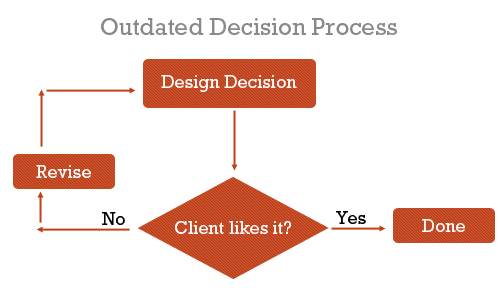
\includegraphics[scale=0.8]{OutDatedDecisionProcess.jpg}
\caption{old decision process, Jacob Gube 2010}
\end{figure}
Nowhere in the design process was the users a factor, the design was simply made according to how the designers as well as the client felt it should be. Making the same kind of chart for a user-centred approach would look like this:\\
\begin{figure}[H]
\centering
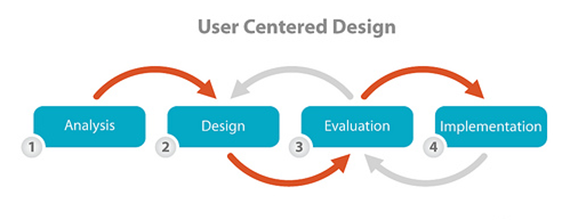
\includegraphics[scale=0.8]{UserCenteredDesign.png}
\caption{a chart of how user-centered design could function, Usabilla 2014}
\label{UXUserCentred}
\end{figure}
As this chart shows, user-centred design can be an iterative process. The grey arrows represents the user feedback, which shows that the users should be involved 
in the evaluation of a design.

User Experience and usability is often confused since a large portion of the guidelines for proper usability also applies to giving a good user experience. 
What sets the user experience apart from usability is that UX deals with the feeling of usage and usability deals with the effectiveness of usage
\todo{source for the example}An example of which could be the iBooks app for iPhone and iPad, an application for reading and browsing E-books.
\begin{figure}[H]
\centering
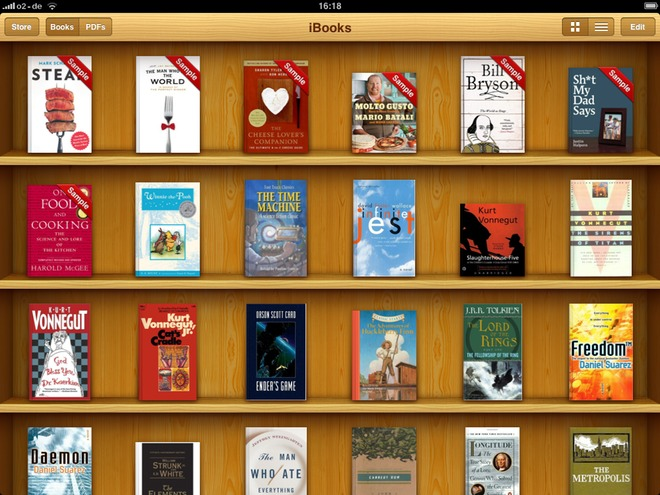
\includegraphics[scale=0.5]{iBooks.png}
\caption{Apple iBooks for comparison}
\end{figure}\todo{might need a source reference}

\begin{figure}[H]
\centering
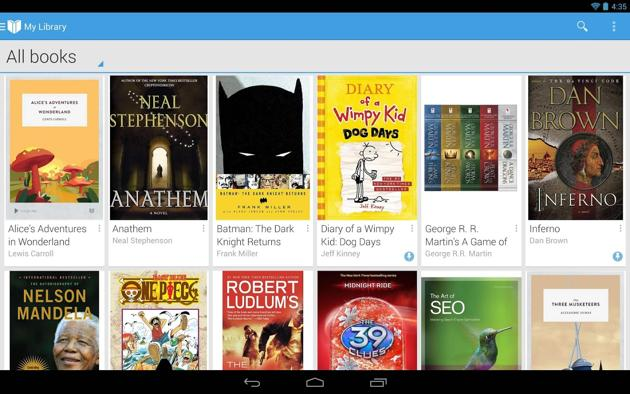
\includegraphics[scale=0.5]{GooglePlayBooks.png}
\caption{Google Play Books for comparison}
\end{figure}\todo{might need a source reference}
The layout is simple, it provides an overview of the owned books with a visual representation of the 
covers which is common for such apps and thus, it does not set itself apart from the state of the art when it comes to usability. However the user experience is 
greatly improved simply by changing the background to resemble a bookshelf, it makes the experience of logging onto iBooks resemble the experience of going into a book store or library a lot more. This approach relates to the concept of 
intuition as familiarity, which will be discussed in the next section.    
\subsection{Intuitiveness is familiarity} \label{IntuIsFam}
As explained in the previous section \ref{UXIntro} user centred design is a main 
pillar of user experience. This is even more true when talking about intuition as 
a design concept. As Jared M. Spool mentions in his 2005 article \textit{People 
Intuit, not Interfaces}\cite{JaredMSpool} the article mentions that it is the 
users that define whether or not an interface is intuitive, as the interface 
itself is nothing more than a collection of code. What this shows is that for an 
interface to be intuitive, a comprehensible knowledge about the targeted users' 
previous experience with similar interaction, is not only useful but absolutely 
crucial. The article introduces the concept of a knowledge space, which is the 
arbitrary space that holds all the knowledge that pertains to a given interface. 

\begin{figure}[H]
\centering
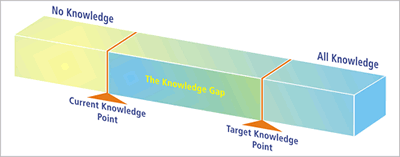
\includegraphics[scale=1]{KnowledgeSpace.png}
\caption{The knowledge space viewed as a continuous curve going from \textit{no 
knowledge} to \textit{all knowledge} \cite{JaredMSpool}}
\label{fig:Knowledge}
\end{figure}

As seen in figure: \ref{fig:Knowledge} there are two points of interest in the 
knowledge space that is the \textit{Current Knowledge Point} and the 
\textit{Target Knowledge Point}. A brief explanation of the two points:
\begin{description}
 \item[\textbf{Current Knowledge Point}] \hfill\\
This is the expected user knowledge which can be defined by a multitude of ways i.e. user interviews, analysis of similar apps etc. Figuring out what the 
current knowledge point is will enable the app to fill the knowledge gap without 
having to guide the user through every tiny detail. 
\item[\textbf{Target Knowledge Point}]\hfill\\
This is the amount of knowledge a user needs to be able to use the app/programme
as intended.
\item[\textbf{The Knowledge Gap}]\hfill\\
The knowledge gap is all the knowledge that the app/programme will have to 
provide for the user. This is usually done with a series of tutorials. 
\end{description}

He puts forth two conditions which he determines are the ones needed 
before users will classify an interface as being intuitive. These are:
\begin{itemize}
\item \textit{Both the current knowledge point and the target knowledge point are 
identical. When the user walks up to the design, they know everything they need 
to operate it and complete their objective.}
\item \textit{The current knowledge point and the target knowledge point are 
separate, but the user is completely unaware that the design is helping them bridge 
the gap. The user is being trained but in a way that seems natural.}
\end{itemize}\label{intuitiveConditions} 
Of these two conditions the latter one will probably be of more use to the 
project as the navigation with the gyroscope will not be a control scheme that 
the user necessarily  have used before. Since the end product is going to 
introduce an uncommon way of interacting, it will be important to know which kind 
of interaction will feel most familiar for the user. This is where the iterative 
process will enable extensive testing of different interaction models, to 
determine the correct approach for our users.
\subsubsection{Flow through the knowledge gap}
\label{FlowTheory}

As Mihaly Csikszentmihalyi \cite{Flow} explains it; for the user to experience a state of flow, the goal and the progress towards it must be clear and well defined as this will be one of the most driving factors when trying to reach this state. The goal should be not too difficult nor too easy but perfect for the user's skill. Just enough to provide the perfect balance between user's skill and the challenges given.\cite{Flow}
	
The real experience begins with when one uses all the concentration on task or challenge at hand making user more and more focused until the user "steps out" of his reality. This is when the state of flow is being reached. \cite{Flow} During this state the user may only feel restricted to the rules of the activity instead of the ones in reality. This can also be called a loss of self awareness. During this state the user may loose sense of time or even one's bodily needs if state of flow is very strong.\cite{Flow}
	
To maintain the state of flow receiving immediate feedbacks step by step on how the user is doing is to be established in order to adjust the challenges and skill level necessary to achieve upcoming goals. \cite{Flow} 

This theory will be used to support and enhance the user's experience when navigating in 3D environment. This will be done by making the challenge given, in this case navigation, challenging for the user yet still balanced in terms of skill that is required to successfully finishing the given task. If successfully implemented, this should establish the state of flow. \cite{Flow} 
\subsection{Designing intuitively}
The topics discussed in the previous section \ref{IntuIsFam} helps define what the app has to be 
able to do but besides these ideas and topics the project will look at the following two structures that can help create a pleasant UX:
\begin{itemize}
\item  Empowering Users to Complete Tasks Faster\\
 \textit{“When a user has a good experience, one of the first things they say 
 that they liked about it is that it was fast. Since users "equate fast with 
 easy," }.\cite{UXKeys} The app that this project will develop does not contain a 
 wide range of features but is a relatively specialized app. While this 
 diminishes the urgency of the app being fast, it should not be neglected. \label{EvalConFast}
 Robinson points to 6 ways of empowering the users effectiveness\cite{UXKeys}:
 \begin{enumerate}
 \item \textbf{Make the app work faster}\\
 This is a straight forward engineering problem as better/less code results in a 
 faster interface. 
 \item \textbf{Simplify your users’ work flow}\\
  This means cutting down on the amount of screens that the app employs.
 \item \textbf{Make sure your navigation is intuitive}\\\label{effectivenessP3}
 As talked about earlier, intuition is related to familiarity and should be able to provide an 
 intuitive navigation within the app.
 \item \textbf{Reduce the amount of text}\\
 In relation to the second point, if an app has a lot of text it will slow down 
 the work flow of the user, at least in the beginning.
 \item \textbf{Examine your graphics}\\
 Robinson points to graphics as being an important part of how a user perceives 
 an app, she urges to keep the graphics: \textit{"clean and not distracting"} 
 \item \textbf{Buttons}\\
 When making any kind of button make sure that the user never questions whether 
 or not it is a button. Furthermore, Robinson also encourages to give the buttons one-word labels such as "send", "buy", "find" etc. Of course the words should 
 represent the action that the button performs.
 \end{enumerate} 
\end{itemize} 
These points together with the intuitiveness discussion above should enable the 
app to provide an intuitive user experience. 

\subsection{Usability}
\label{Usability}

According to John Wiley's "Interaction design", there are usability goals that are worth considering when developing interactive and usable systems \cite{Wileys} The covered usability goals are:

\begin{itemize}
\item Effective to use\\
The system does what it suppose to do.
\item Efficient to use\\
The system supports the user while interacting	
with it.
\item Safe to use
\item Good utility \\
Provides variety of functionality that the user might need.
\item Easy to learn
\item Easy to remember how to use
\end{itemize}


Wiley notes that not all of the goals are needed for most of the systems \cite{Wileys}. Specific systems should have specific goals. Probably the most important and relevant goals for this application design is effectiveness and efficiency. In order to help the user navigate in the 3D environment, this system has to have an accurate response which saves time and does tasks quickly. E.g. if the user wants to view 3D objects from a certain angle, it is easy and fast to navigate to the point where the view angle is desired. For the beginners of such interaction with 3D environments, "easy to learn" and "easy to remember" goals would be most relevant. Don Norman states in his "The Design of Everyday Things" that there is a principle of "affordance". \cite{Normans} The principle is being explained as e.g. A cup is affordable for being picked up, a door is affordable of being opened because of its doorknob, a button affords being pressed etc. So if the user is at a beginner level, the principle of "affordance" is extremely useful.Norman in "The Psychology of Everyday Things" notes that there are two "affordances"; real and perceived \cite{Affordance}. Real is the one in real world as in examples mentioned above and perceived is imitation of reality. E.g. in this design, for beginners especially, navigation buttons needs to look very similar to "real" navigation buttons. For instance, if the user is familiar with any common video gaming console buttons, they have to be represented in a interactive software system with similarity to real one. 

Don Norman also covers other principles of usability:\cite{Normans}
\begin{itemize}
\item Visibility\\
How visible is the button on the screen?
\item Feedback\\
What kind of feedback does the system gives to the user?
\item Constrains\\
Visual constraints as e.g. graying out some menu which is not used.
\item Mapping \\
Layout of menus, buttons etc.
\item Consistency\\
Consistency through the system in layouts, colors, typography etc.
\item Affordance\\
Real and perceived affordance, covered above.
\end{itemize}

Like with usability goals not all of the principles of usability needs to be in 
one system. However, in this case, the design of the program can include all 
mentioned principles. E.g. if the 3D navigation system is controlled by the 
buttons on the screen, they need to be visible, give   feedback when 
pressed, mapped out with consistency rules and visualized with "affordance" 
principle. 

\subsubsection{Mobile Usability}
\label{MobileUsability}

Since the design of this system is meant to be on a mobile platform, there are certain aspect to consider. Some users might have limited mobility or problems with manual dexterity - it will cause higher error rates with the interaction \cite{Wileys}. Even small aspects like a person's big fingers can cause problems while using a cellphone and especially while interaction needs precision. This problem is mentioned in many articles, reports, researches. In "The Generalized Perceived Input Point Model and How to Double Touch Accuracy by Extracting Fingerprint" \cite{Fatfinger} where they introduce possible solutions to this problem. Since the focus of this project is not solving such problems, a deeper analysis will not be done. Some considerations might be done as using Norman's principle of feedback.\cite{Normans} Buttons pressed on a screen can change the color or the size. Mobile devices could use some sensors to indicate that the action is achieved, as vibration, blinking flash etc. It is especially useful since most smartphones using on-screen touch buttons and physical sensation of touching the button is non-existing.  The user who did not register if he successfully completed the wanted action should get feedback from the mobile device. Feedback is also useful to people who do not put lots of attention to their interaction accuracy; pressing somewhere around button areas and not on it. Feedback would help users to know if a specific action is successful. 
In general, it is important to consider minorities and helping users effectively understand the efficiency of their actions. Since this non-traditional interaction method can be used by many people which was discovered in analysis of target group, \ref{TargetGroup} product needs to be optimized to at least fit majority of the users. 

\subsection{conclusion}
This section has aimed at defining the intuitive user experience which has been defined to be a fulfillment of one of the two conditions mentioned on page \pageref{intuitiveConditions}. The section has also showed that intuitiveness depends on both the users previous knowledge, as well as the design of the interface. Considering Norman's and Wiley's usability goals and principles, it is 
possible to create a useful application. Usability goals of effectiveness and 
efficiency will be achieved by using all covered principles. Principles will be 
used in creation of visual elements and coding. Having goals as "easy to learn and 
remember" will help to narrow the knowledge gap when the users first encounter the app/programme. A solution to that is to create interactive navigation using the
affordance principle and visual familiarity.\label{EvalConUsability}
